\documentclass[tikz, multi=page]{standalone}
\usepackage{../tikz-preamble}
\usepackage{pdfpages}
\usepackage{blkarray}

% arara: pdflatex: { synctex: no }
% arara: latexmk: { clean: partial }
\begin{document}

\begin{page}
\begin{tikzpicture}[bend angle=20]

    \node[state] (0) {0};
	\node[state] (1) [right = of 0] {1};
	\node[state] (2) [right = of 1] {2};
	\node[state] (3) [below = 2.5cm of 0] {3};
	\node[state] (4) [right = of 3] {4};
    \node[state] (5) [right = of 4] {5};

	\path[di] (0) edge node {} (1);
	\path[di] (0) edge[bend right] node {} (3);
	\path[di] (3) edge[bend right] node {} (0);
	\path[di] (1) edge node {} (2);
	\path[di] (1) edge node {} (2);
	\path[di] (2) edge node {} (3);
	\path[di] (3) edge node {} (4);
    \path[di] (4) edge node {} (2);

\end{tikzpicture}
\end{page}

\begin{page}\Large
\begin{blockarray}{ *{7}{ >{\bfseries}c } }
	& 0 & 1 & 2 & 3 & 4 & 5 \\[5pt]
	\begin{block}{ >{\bfseries}c @{\hspace{20pt}} ( *{6}{c} ) }
		0 & 0 & 1 & 0 & 1 & 0 & 0 \\
		1 & 0 & 0 & 1 & 0 & 0 & 0 \\
		2 & 0 & 0 & 0 & 1 & 1 & 0 \\
		3 & 1 & 0 & 0 & 0 & 1 & 0 \\
		4 & 0 & 0 & 1 & 0 & 0 & 0 \\
		5 & 0 & 0 & 0 & 0 & 0 & 0 \\
	\end{block}
\end{blockarray}
\end{page}

\begin{page}
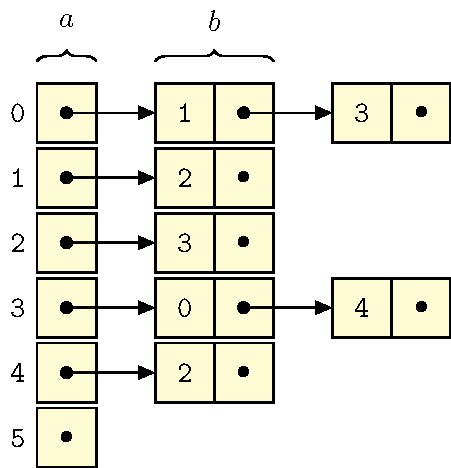
\includegraphics{memory1}
\end{page}

\begin{page}
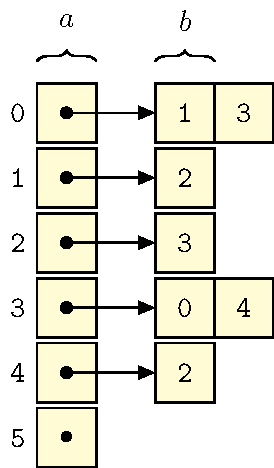
\includegraphics{memory3}
\end{page}

\end{document}
